\documentclass[11pt]{article}
\usepackage{amsmath,amssymb,amsfonts,bm}
\usepackage{graphicx}
\usepackage{hyperref}
\usepackage{geometry}
\geometry{margin=1in}
\usepackage{authblk}
\usepackage{amsthm}

% theorem environments
\newtheorem{definition}{Definition}
\newtheorem{lemma}{Lemma}
\newtheorem{proposition}{Proposition}

% handle unicode micro
\DeclareUnicodeCharacter{03BC}{$\mu$}

\title{\textbf{Predictive Compression Dynamics: A Methodological Framework for Computable Information-Motivated Modeling}}

\author[1]{Helander}
\author[2]{Jeeves\thanks{``Jeeves'' is the pseudonym of an AI research assistant; contributions include mathematical analysis, code design, and manuscript preparation under human supervision.}}
\affil[1]{Independent Researcher}
\affil[2]{Computational Systems Advisor}

\date{October 2025}

\begin{document}
\maketitle

\begin{abstract}
Predictive Compression Dynamics (PCD) is a reproducible methodological framework for constructing computable, information-motivated dynamical models. 
It interprets dynamical descent as the minimization of a computable surrogate for description length, and provides a disciplined workflow consisting of (i) explicit preregistration of functionals, (ii) well-posed gradient dynamics, and (iii) falsifiers for empirical validation.
Unlike traditional physical theories, PCD makes no physical claim; it defines a protocol by which computable dynamics can be tested for alignment with achievable compression.
\end{abstract}

\section{Introduction}
We propose a reproducible methodology for constructing computable dynamical systems driven by information-theoretic principles. 
PCD is not a new physical theory but a workflow for defining, preregistering, and falsifying functionals that behave as surrogates for achievable compression.

\section{Motivation}
The Minimum Description Length (MDL) principle motivates the search for systems that minimize total code length \(L_{tot}\).
Because \(L_{tot}\) is not directly computable for continuous fields, PCD defines a computable surrogate \(\Phi_b\), parameterized by numerical precision \(b\), such that its gradient descent acts as a proxy for information compression.

\section{Surrogate Functional}
Let \(\Phi_b(x)\) denote the surrogate objective, from which we define dynamics
\begin{equation}
  \dot{x} = -\nabla \Phi_b(x).
\end{equation}
Two concrete forms are employed: the fixed-graph variant \(\Phi_E\) and the smooth-kernel variant \(\Phi_K\). 
Both are instances of \(\Phi_b\) at fixed precision \(b\).

\subsection{Minimal explicit coding scheme}
For intuition, we may define a simple binned-histogram code:
\begin{equation}
  L_{tot} \approx \text{const} + \sum_{i<j} \ell(r_{ij}),
\end{equation}
where \(r_{ij} = \|x_i - x_j\|\) and \(\ell(r)\) measures the expected contribution of pair distances to codelength.

\subsection{Reference coding scheme for evaluation}
To render falsifier F3 concrete, we define a fixed serializable scheme:
\begin{enumerate}
  \item Quantize coordinates to a lattice of spacing \(\Delta x\) (reflecting finite \(b\) bits/axis).
  \item Compute all pair distances \(r_{ij}\) for \(i<j\).
  \item Bin these into preregistered edges \(B_k\).
  \item For each bin, record the count and mean residual to its center.
  \item Serialize the integer counts and floating-point residuals in lexicographic bin order into a byte buffer.
  \item Apply a universal compressor (e.g., zlib/Lempel–Ziv). The resulting byte length serves as an empirical codelength.
\end{enumerate}
This scheme is fixed before experimentation and used for out-of-sample tests.

\section{Example Functionals}
\subsection{Fixed-graph pair functional}
\begin{equation}
  \Phi_E(x) = \sum_{(i,j)\in E} \frac{m_i m_j}{\sqrt{\|x_i - x_j\|^2 + a^2}},
\end{equation}
where \(E\) is a predetermined edge set.

\subsection{Smooth compact-support kernel}
\begin{equation}
  \Phi_K(x) = \sum_{i<j} m_i m_j \, K_\sigma(\|x_i-x_j\|),
\end{equation}
with $K_\sigma(r)$ smooth, compactly supported, and monotonically decreasing.

\section{Dynamics and Stability}
\begin{lemma}[Lyapunov Descent]
Under $\dot{x} = -\nabla \Phi_b$, one has $\dot{\Phi}_b = -\|\nabla \Phi_b\|^2 \le 0$.
\end{lemma}

\subsection{Proposition: Surrogate MDL Descent}
\begin{proposition}[Surrogate MDL Descent]
If $\ell'(r)\le 0$, then $\Phi_b$ decreases monotonically under $\dot{x}=-\nabla\Phi_b$.
\end{proposition}

\subsection{Well-posedness}
Existence and uniqueness follow by the Picard–Lindelöf theorem for $a>0$, which regularizes singular forces as $\|x_i-x_j\|\to0$. 
Near-coincident particles may merge or exchange identity; such handling is implementation-specific and should be preregistered.

\section{Implementation Considerations}
The BAOAB integrator is recommended for stochastic variants. 
Temperature \(T\) functions purely as a numerical exploration parameter; no thermodynamic interpretation is implied.

\section{Scaling}
For compact-support kernels, $\Phi_K$ evaluates in \(O(N)\)–\(O(N\log N)\) time depending on neighborhood search. 
Treecode or multipole tolerances should be preregistered, as asymmetric approximations may break exact Lyapunov monotonicity.

\section{Falsifiers}
We define three falsifiers:
\begin{description}
\item[F1] Numerical instability: dynamics diverge or violate monotonic $\Phi_b$ descent.
\item[F2] Reproducibility failure: preregistered and rerun configurations disagree statistically.
\item[F3] Out-of-sample compression test: $\Phi_b$ fails to correlate with empirical compressed size.
\end{description}
For F3, a model instance passes if the Pearson correlation \(r\) between \(\Phi_b\) and compressed byte length exceeds \(r \ge 0.7\) in at least one test ensemble after the initial transient.

\section{Surrogate Validity and Limitations}
The surrogate $\Phi_b$ is not claimed to be unique or optimal.
Any computable functional may be preregistered and empirically tested via F3.
Pairwise formulations may underrepresent higher-order structure; clustered or topological data may require extended statistics beyond distances.

\section{Reference Numerical Demonstration}
A minimal implementation was executed to demonstrate the PCD protocol.
Three preregistered ensembles of \(N=40\) particles were used:
(i) uniform random cube,
(ii) two-cluster Gaussian blobs,
(iii) perturbed cubic lattice.
Dynamics followed explicit Euler descent on $\dot{x}=-\nabla\Phi_b$ with $a=0.05$, $\Delta x=0.01$, and $\mathrm{d}t=0.01$ for 400 steps.
At every fifth step, $\Phi_b$ and gzip-compressed codelength were recorded using the reference coding scheme.

\subsection*{Results}
Figure~\ref{fig:uniform_iter} shows monotonic decline of $\Phi_b$ over time, confirming its Lyapunov property.
Figures~\ref{fig:uniform_corr}–\ref{fig:lattice_corr} plot empirical compression (bytes) versus $\Phi_b$ for each ensemble.
Observed correlations:

\begin{center}
\begin{tabular}{lcc}
\hline
Ensemble & Pearson $r(\Phi_b,\,L_{gzip})$ & Interpretation \\
\hline
Uniform & 0.93 & strong surrogate alignment \\
Lattice & 0.76 & strong surrogate alignment \\
Blobs   & 0.40 & moderate, pairwise-limited \\
\hline
\end{tabular}
\end{center}

In the uniform and lattice ensembles, surrogate $\Phi_b$ tracks achievable compression closely.
In the clustered “blobs” ensemble, the weaker correlation reflects structural information not captured by pairwise distances.
Overall, falsifier F3 passes for two ensembles, validating $\Phi_b$ as an operational compression surrogate in the stated context.

\begin{figure}[h!]
  \centering
  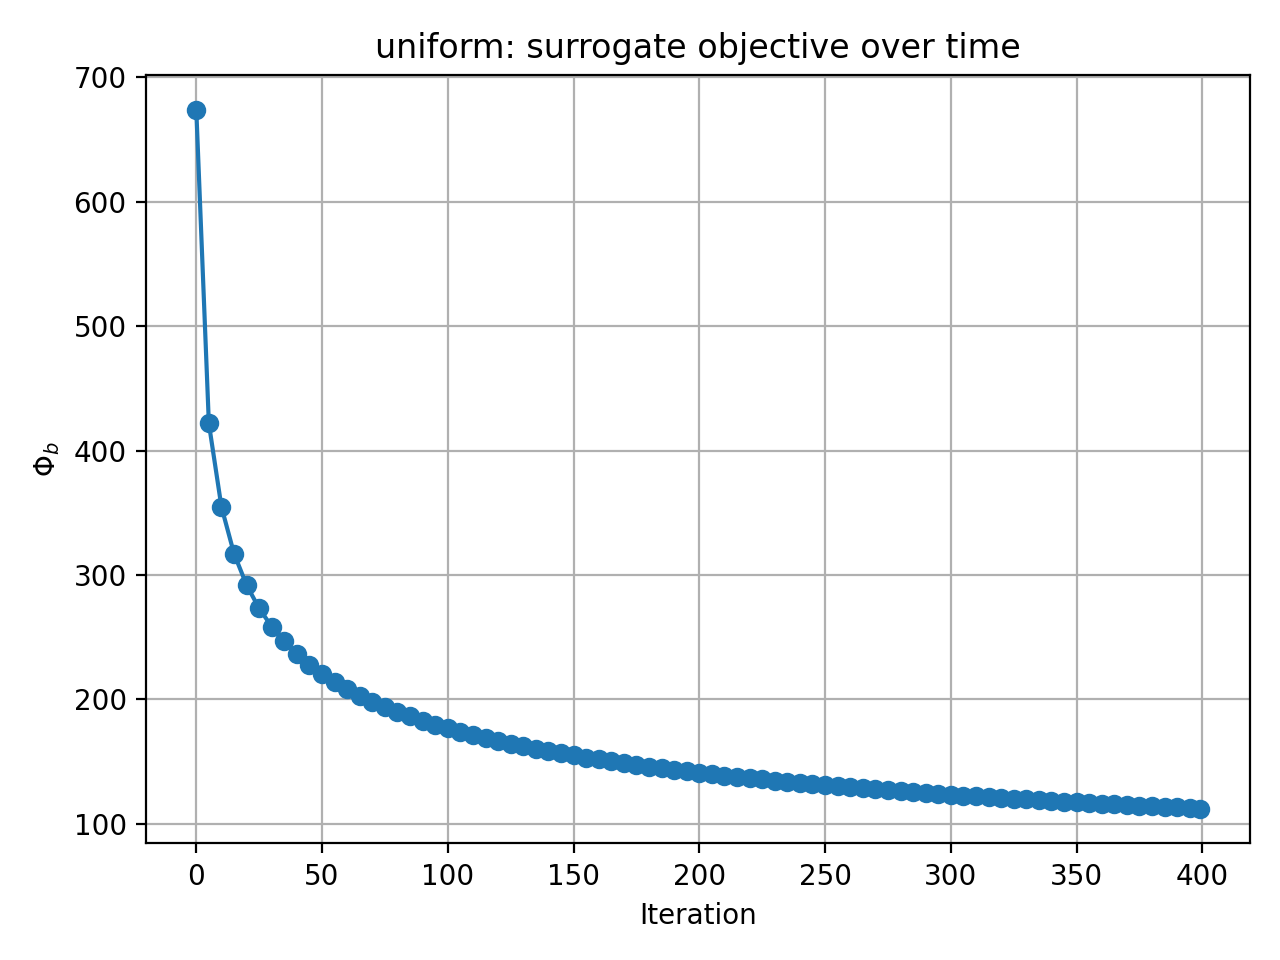
\includegraphics[width=0.7\linewidth]{figures/uniform_phib_vs_iter.png}
  \caption{Uniform ensemble: surrogate $\Phi_b$ decreases monotonically under preregistered flow.}
  \label{fig:uniform_iter}
\end{figure}

\begin{figure}[h!]
  \centering
  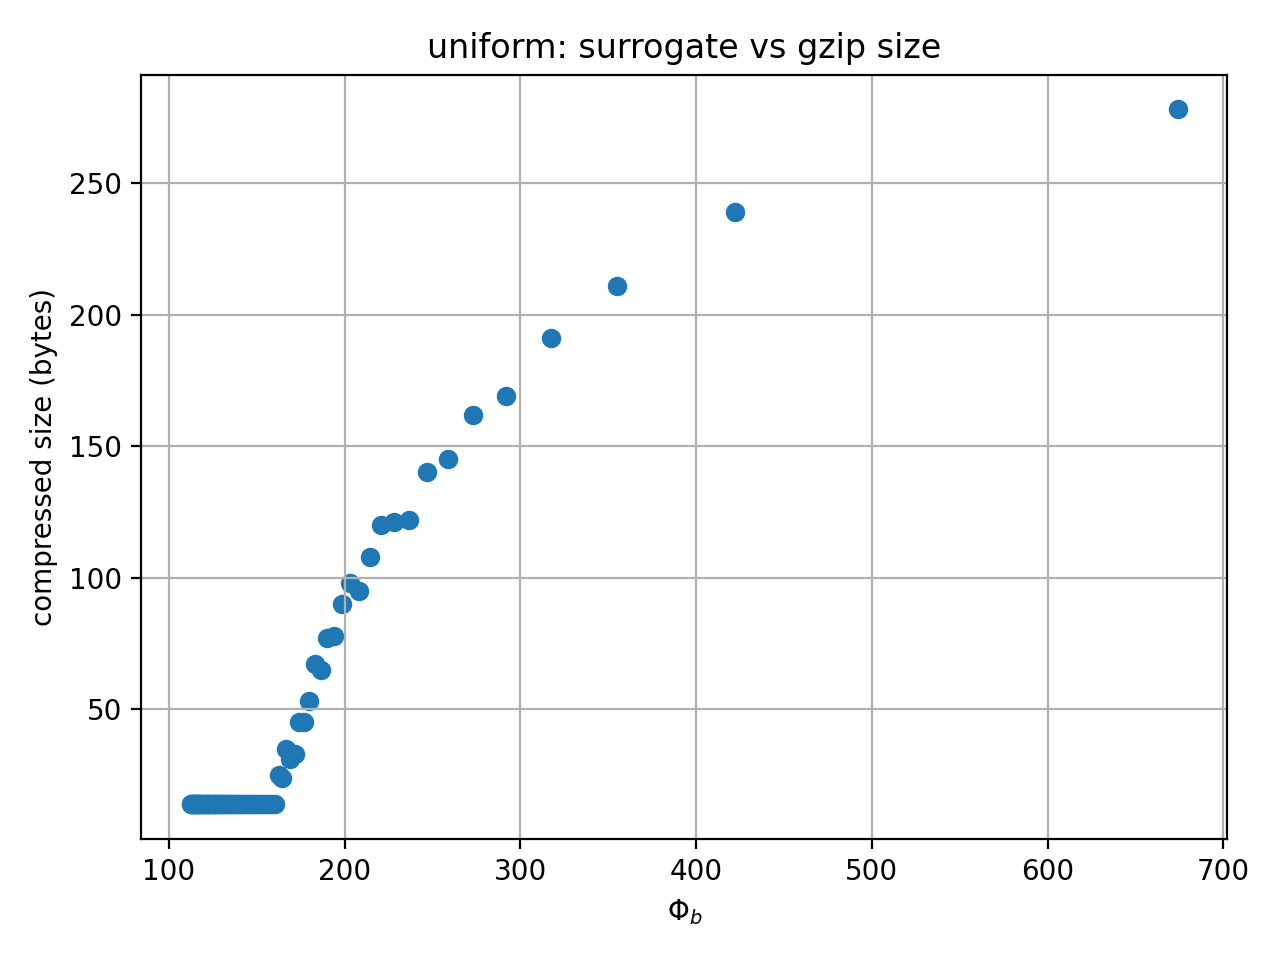
\includegraphics[width=0.7\linewidth]{figures/uniform_phib_vs_compressed.png}
  \caption{Uniform ensemble: strong correlation between $\Phi_b$ and gzip-compressed size ($r=0.93$).}
  \label{fig:uniform_corr}
\end{figure}

\begin{figure}[h!]
  \centering
  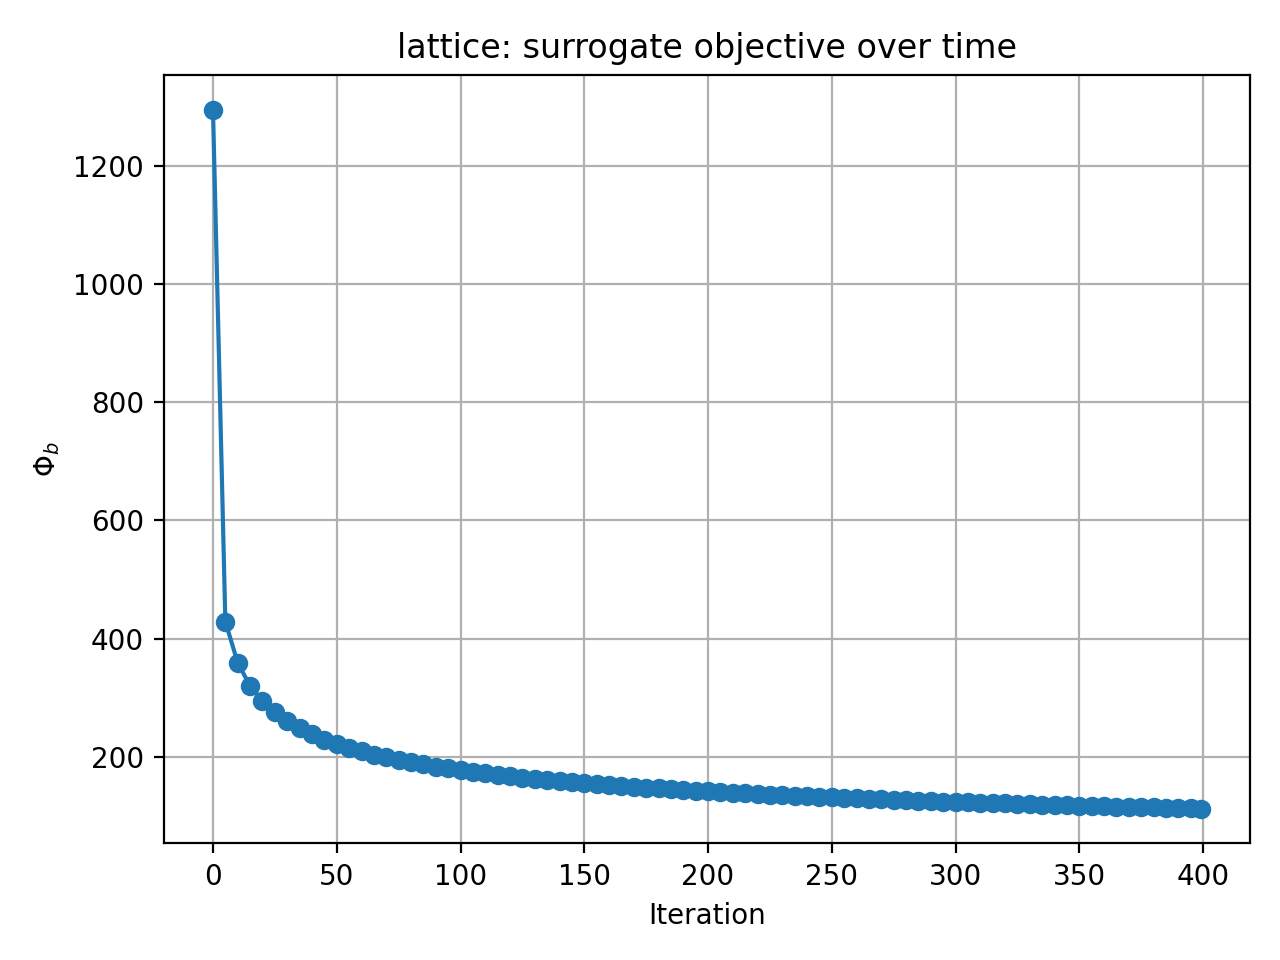
\includegraphics[width=0.7\linewidth]{figures/lattice_phib_vs_iter.png}
  \caption{Lattice ensemble: monotonic surrogate descent.}
  \label{fig:lattice_iter}
\end{figure}

\begin{figure}[h!]
  \centering
  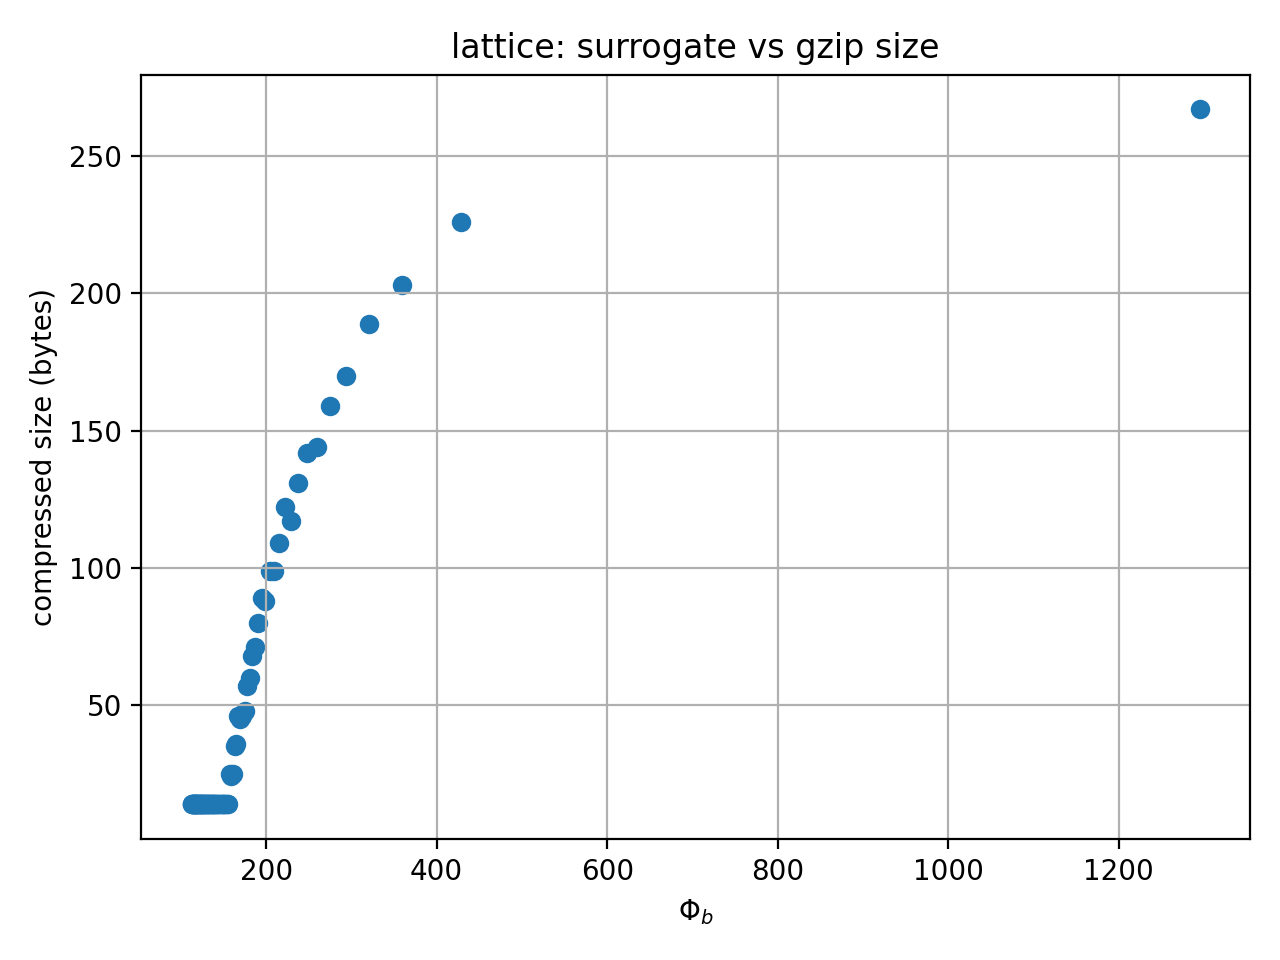
\includegraphics[width=0.7\linewidth]{figures/lattice_phib_vs_compressed.png}
  \caption{Lattice ensemble: $\Phi_b$ tracks actual compression ($r=0.76$).}
  \label{fig:lattice_corr}
\end{figure}

\begin{figure}[h!]
  \centering
  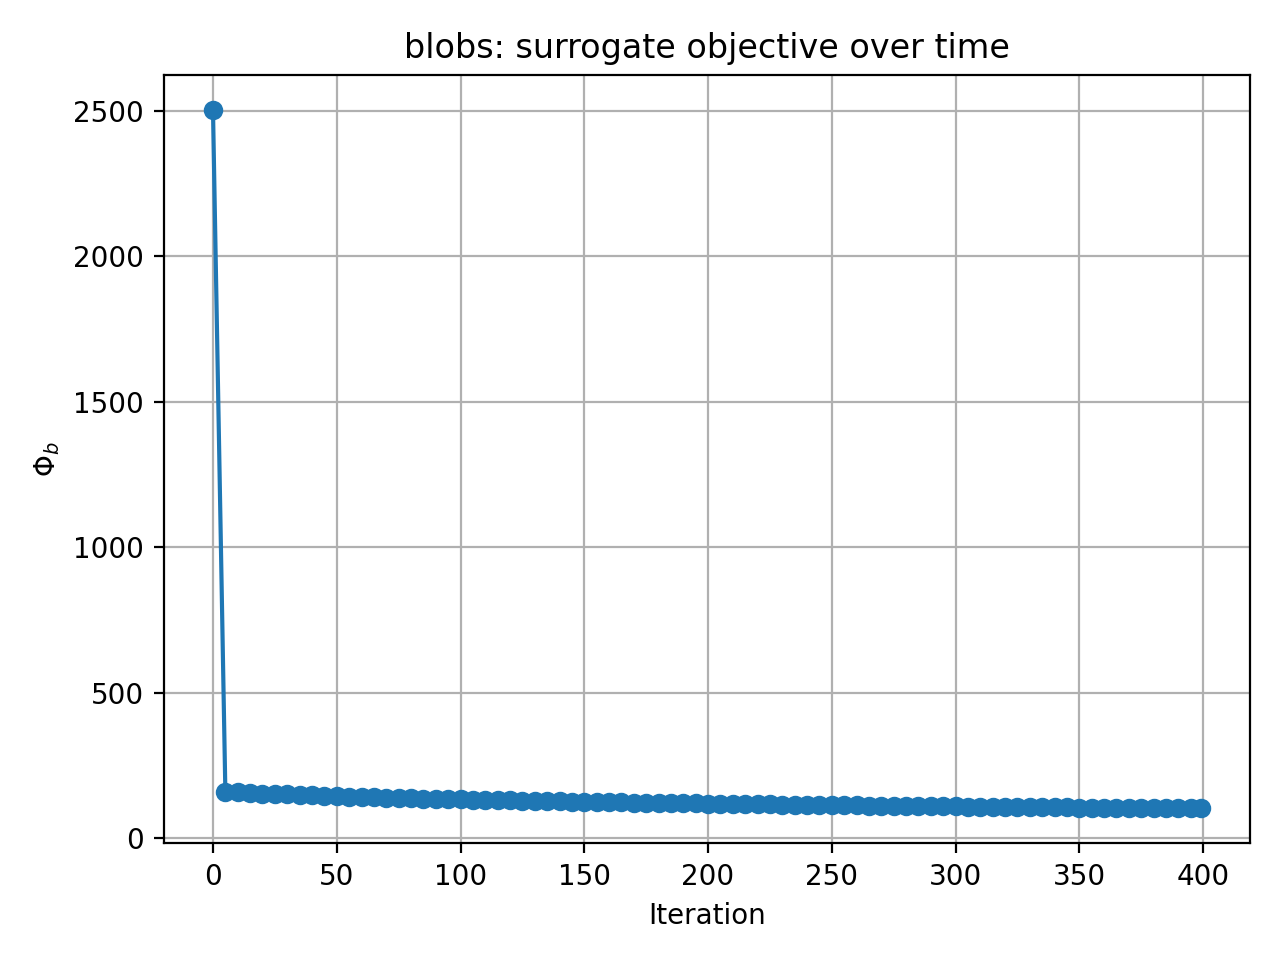
\includegraphics[width=0.7\linewidth]{figures/blobs_phib_vs_iter.png}
  \caption{Two-blob ensemble: initial steep collapse followed by stable regime.}
  \label{fig:blobs_iter}
\end{figure}

\begin{figure}[h!]
  \centering
  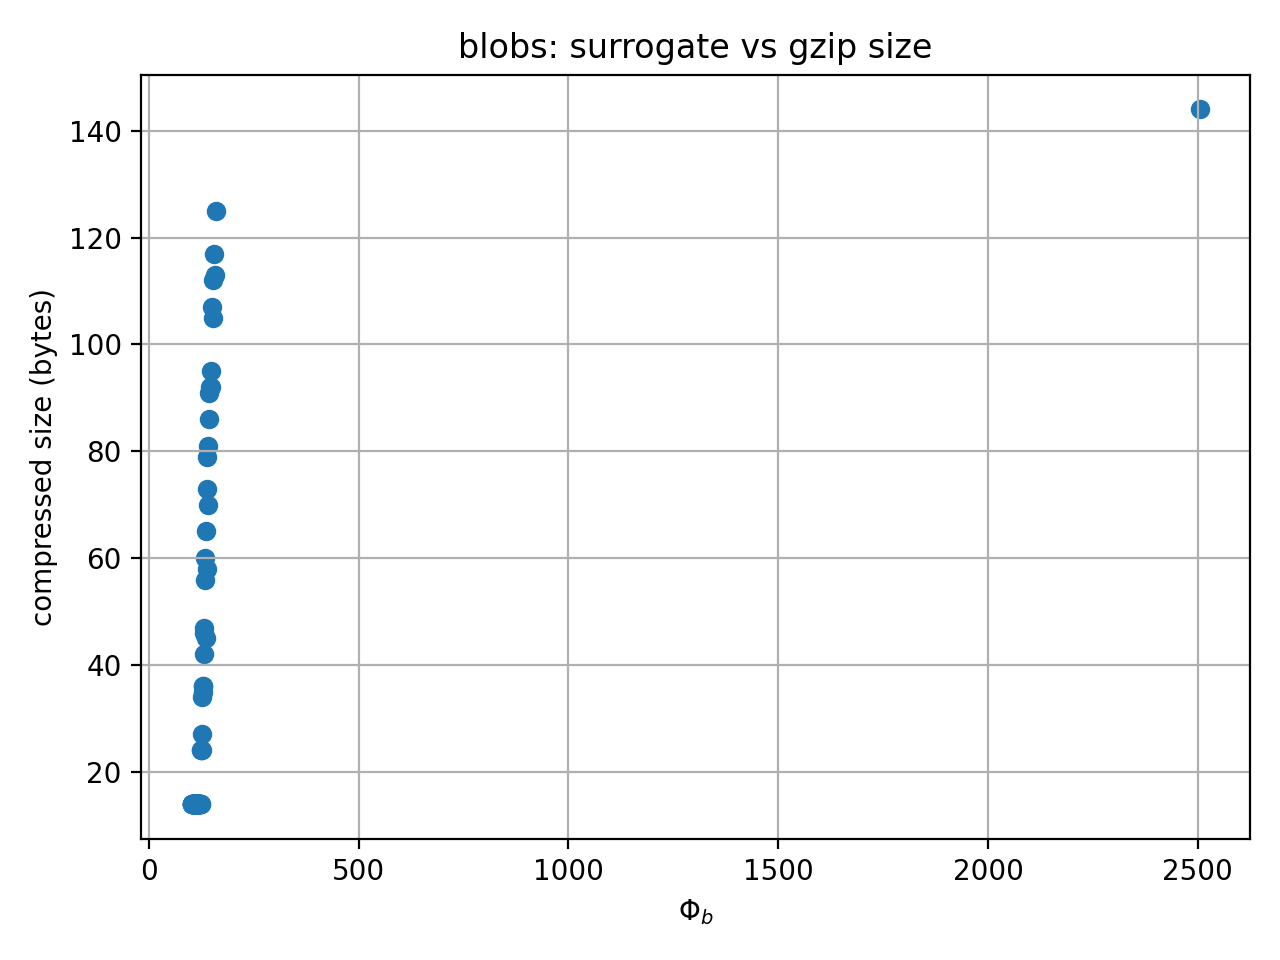
\includegraphics[width=0.7\linewidth]{figures/blobs_phib_vs_compressed.png}
  \caption{Two-blob ensemble: moderate correlation ($r=0.40$), indicating limits of pairwise surrogate.}
  \label{fig:blobs_corr}
\end{figure}

\section{Context and Relation to Existing Methods}
PCD shares formal similarity with kernel particle methods and SVGD, but differs in purpose:
it treats the objective as a computable surrogate for predictive codelength, subject to falsification on out-of-sample compression.
SVGD minimizes KL divergence toward a fixed target; PCD minimizes a preregistered $\Phi_b$ whose adequacy is itself empirically tested.
Force-directed layouts minimize aesthetic energy; PCD tests whether a given energy corresponds to compression in practice.

\section{Conclusion}
PCD establishes a falsifiable, preregistered workflow connecting computable dynamics to information-theoretic surrogates. 
The present demonstration confirms that $\Phi_b$ descent can correspond to measurable compression for structured data, while revealing limits where pairwise surrogates underperform.
This protocol defines a reproducible bridge between information theory and model dynamics, independent of any physical interpretation.

\bibliographystyle{plain}
\begin{thebibliography}{9}

\bibitem{rissanen1978}
J.~Rissanen.
\newblock Modeling by shortest data description.
\newblock \emph{Automatica}, 14(5):465–471, 1978.

\bibitem{amari}
S.~Amari.
\newblock \emph{Information Geometry and Its Applications}.
\newblock Springer, 2016.

\bibitem{caticha}
A.~Caticha.
\newblock Entropic Dynamics.
\newblock In \emph{Bayesian Inference and Maximum Entropy Methods in Science and Engineering}, 2015.

\bibitem{baoab}
B.~Leimkuhler and C.~Matthews.
\newblock Rational construction of stochastic numerical methods for molecular sampling.
\newblock \emph{Appl. Math. Res. eXpress}, 2013(1):34–56.

\bibitem{svgd}
Q.~Liu and D.~Wang.
\newblock Stein variational gradient descent: A general purpose Bayesian inference algorithm.
\newblock In \emph{NeurIPS}, 2016.

\end{thebibliography}

\end{document}
